\documentclass[12pt]{scrartcl}
\usepackage{fullpage,enumitem,amsmath,amssymb,graphicx}

\addtokomafont{section}{\normalsize}
\setlength{\parindent}{0pt}

\newcommand{\vect}[1]{\boldsymbol{#1}}
\newcommand{\ve}{\vect}
\newcommand\R{\mathbb{R}}
\newcommand\E{\mathbb{E}}
\newcommand{\fx}[1]{#1(\vect{x})}
\newcommand{\diff}[1]{\,\mathrm{d}#1}

\DeclareMathOperator*{\argmin}{arg\,min}
\DeclareMathOperator*{\argmax}{arg\,max}
\newcommand{\p}[1][\mathrm{p}]{\mathrm{#1}}

\title{\large Machine Learning Exercise Sheet 6}
\subtitle{\Large Optimization}
\author{\large\bfseries Group\_369 \\
        \large Fan \textsc{Xue} -- \texttt{fan98.xue@tum.de} \\
        \large Xing \textsc{Zhou} -- \texttt{xing.zhou@tum.de} \\
        \large Jianzhe \textsc{Liu} -- \texttt{jianzhe.liu@tum.de}}
\date{\large \today}
\begin{document}
  \maketitle
  \vspace{-1cm}
  \noindent\rule{\textwidth}{0.4pt}
  \section*{Problem 4}

  \begin{enumerate}[label=\alph*)]
    \item This statement is false, which can be proved by a counterexample. For that, we need to adopt an inference that the second derivation of a convex function is non-negative.
    We take $f(x)=x^2$ and $g(x)=-x$, both of which are convex funtions, since $\dfrac{\mathrm{d}^{2}f(x)}{\mathrm{d}x^{2}}=2 \ge 0$ and $\dfrac{\mathrm{d^{2}}g(x)}{\mathrm{d}x^{2}}=0 \ge 0$.
    Then we take the composition of the two functions as $h(x)=g(f(x))$, and we have:
    \begin{equation*}
      \frac{\mathrm{d^{2}}}{\mathrm{d}x^{2}}h(x)=-2 \le 0.
    \end{equation*}
    That means $h(x)=g(f(x))$ is non-convex.
    \item This statement is true. We prove it with the definition of convex function. We take $h(x)=g(f(x))$, 
     $\forall x_{1},x_{2}\in \R$ and $t \in (0,1)$, since $f(x)$ is convex we have
    \begin{equation*}
      f\left( tx_{1}+(1-t)x_{2} \right) \le tf\left( x_{1} \right) + (1-t)f\left( x_{2} \right).
    \end{equation*}
    Since $g(x)$ is non-decreasing and convex, we have
    \begin{align}
      g\left(f\left( tx_{1}+(1-t)x_{2} \right)\right) &\le g\left( tf\left( x_{1} \right) + (1-t)f\left( x_{2} \right) \right) \\
      g\left( tf(x_1) + (1-t)f(x_2) \right) &\le tg\left( f(x_1) \right) + (1-t)g\left( f(x_2) \right).
    \end{align}
    Combine (1) and (2), we have
    \begin{align*}
      g\left(f\left( tx_{1}+(1-t)x_{2} \right)\right) &\le tg\left( f(x_1) \right) + (1-t)g\left( f(x_2) \right) \\
      &\Updownarrow \\
      h\left( tx_{1}+(1-t)x_{2} \right) &\le th(x_1) + (1-t)h(x_2),
    \end{align*}
    which proves $h(x)=g(f(x))$ is convex.
  \end{enumerate}

    \section*{Problem 5}
\begin{enumerate}[label=\alph*)]
\item 
By observing the given function $\ve{f}$: 
\[f(x_1, x_2) = 0.5{x_1}^2 + {x_2}^2 + 2x_1 + x_2 + \cos(\sin (\sqrt{\pi}))\]
we can find that it consists of several convex functions. Which means that when we separately find all the $x_n$ that minimize its own function, we find the $\ve{x}^\star$ that minimizes the function $\ve{f}$.
\\
The gradient of f can be computed by followings:
\begin{equation*}
    \begin{pmatrix}
        \displaystyle\frac{\partial{f(x_1, x_2)}}{\partial{x_1}}\\
        \displaystyle\frac{\partial{f(x_1, x_2)}}{\partial{x_2}}
    \end{pmatrix}
     =
    \begin{pmatrix}
        \displaystyle x_1 + 2 \\
        \displaystyle 2x_2 + 1
    \end{pmatrix}
     =0
\end{equation*}
So minimizer $\ve{x}^\star$ is:
\begin{equation*}
\ve{x}^\star =
\begin{pmatrix}
         -2 \\
        \displaystyle -\frac{1}{2} 
    \end{pmatrix}
\end{equation*}
\item
2 steps of gradient descent with leaning rate $\tau = 1$ can be performed by following procedure:
\begin{equation*}
\text{step 1:} 
    \begin{pmatrix}
        \displaystyle x{_1}^{(1)} \\
        \displaystyle x{_2}^{(1)}
    \end{pmatrix}
    =
    \begin{pmatrix}
        \displaystyle x{_1}^{(0)} \\
        \displaystyle x{_2}^{(0)}
    \end{pmatrix}
    -\tau \nabla_{\ve{x}} f\left(\ve{x}^{(0)}\right) \\
    =
    \begin{pmatrix}
        -2 \\
        -1
    \end{pmatrix}   
\end{equation*}
\begin{equation*}
\text{step 2:} 
    \begin{pmatrix}
        \displaystyle x{_1}^{(2)} \\
        \displaystyle x{_2}^{(2)}
    \end{pmatrix}
    =
    \begin{pmatrix}
        \displaystyle x{_1}^{(1)} \\
        \displaystyle x{_2}^{(1)}
    \end{pmatrix}
    -\tau \nabla_{\ve{x}} f\left(\ve{x}^{(1)}\right) \\
    =
    \begin{pmatrix}
        -2 \\
        0
    \end{pmatrix}   
\end{equation*}
Here $\nabla f\left(\ve{x}\right)$ is obtained from \textbf{question a)} above, where
\[\frac{\partial{f(x_1, x_2)}}{\partial{x_1}} = x_1 + 2\] 
\[\frac{\partial{f(x_1, x_2)}}{\partial{x_2}} = 2x_2 + 1\] 

\item
we can try computing two more iteration:
\begin{equation*}
    \begin{pmatrix}
        \displaystyle x{_1}^{(3)} \\
        \displaystyle x{_2}^{(3)}
    \end{pmatrix}
    =
    \begin{pmatrix}
        -2 \\
        0
    \end{pmatrix}
    -1
    \begin{pmatrix}
        -2+2 \\
        0+1
    \end{pmatrix}
    =
    \begin{pmatrix}
        -2 \\
        -1
    \end{pmatrix}   
\end{equation*}
\begin{equation*}
    \begin{pmatrix}
        \displaystyle x{_1}^{(4)} \\
        \displaystyle x{_2}^{(4)}
    \end{pmatrix}
    =
    \begin{pmatrix}
        -2 \\
        -1
    \end{pmatrix}
    -1
    \begin{pmatrix}
        -2+2 \\
        -2+1
    \end{pmatrix}
    =
    \begin{pmatrix}
        -2 \\
        0
    \end{pmatrix}   
\end{equation*}

Obviously, it's an endless loop......Yet we already know that minimizer $\ve{x}^\star$ is:
$\begin{pmatrix}
         -2 \\
        \frac{1}{2} 
 \end{pmatrix}$.

So the answer is, this gradient descent procedure can never converge to the true minimizer $\ve{x}^\star$.\\
To solve this problem, we must change the learning rate. In our case, it has to decrease to get to the minimizer.
\end{enumerate}

    \section*{Problem 6}
The result of the programming task is appended at the end of the file.
    \section*{Problem 7}
\begin{enumerate}[label=\alph*)]
\item
This region S is not a convex region. Because we can find points whose line in between is outside region S. As shown in figure 1, red, green and blue lines are all in this situation.

\begin{figure}[htbp]
\centering
\begin{minipage}[t]{0.48\textwidth}
\centering
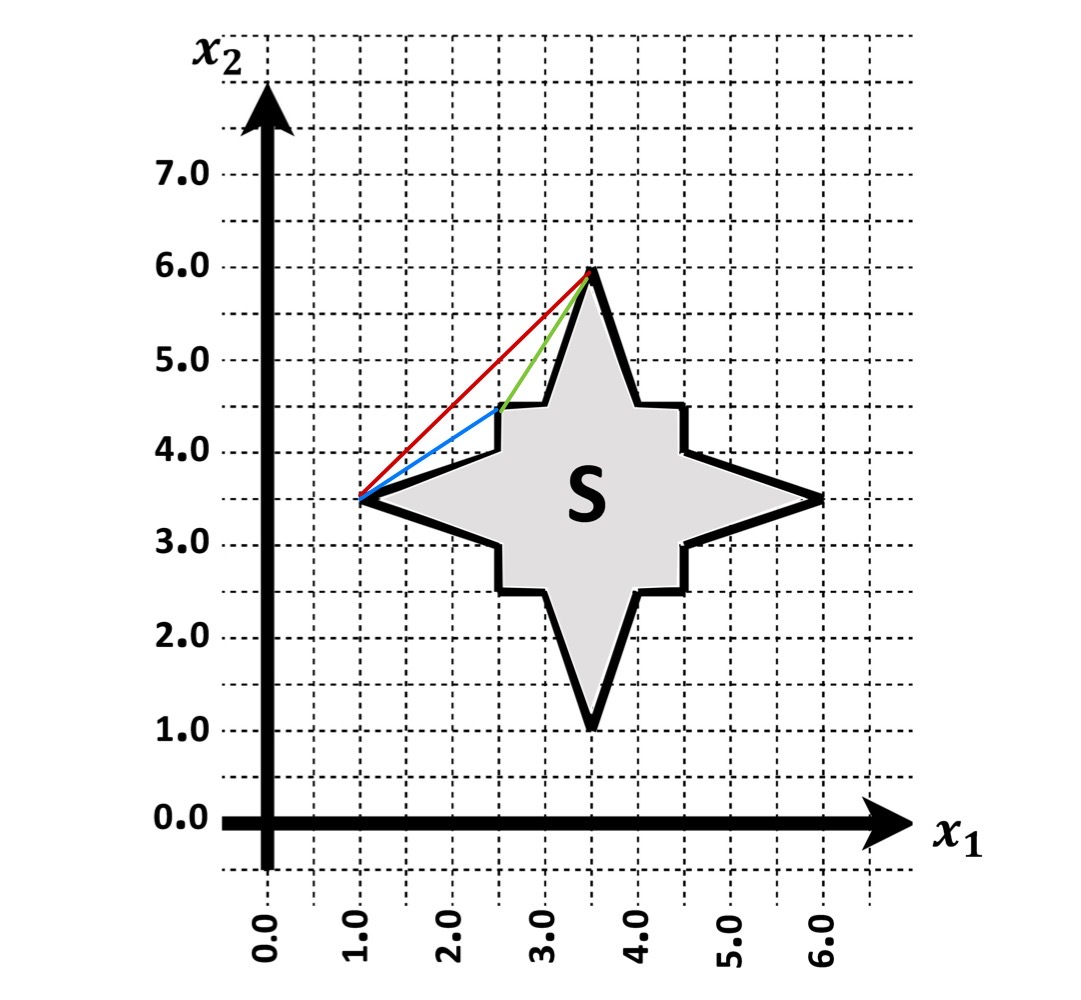
\includegraphics[width=8cm]{Prob7.1.JPG}
\caption{Figure 1}
\end{minipage}
\begin{minipage}[t]{0.48\textwidth}
\centering
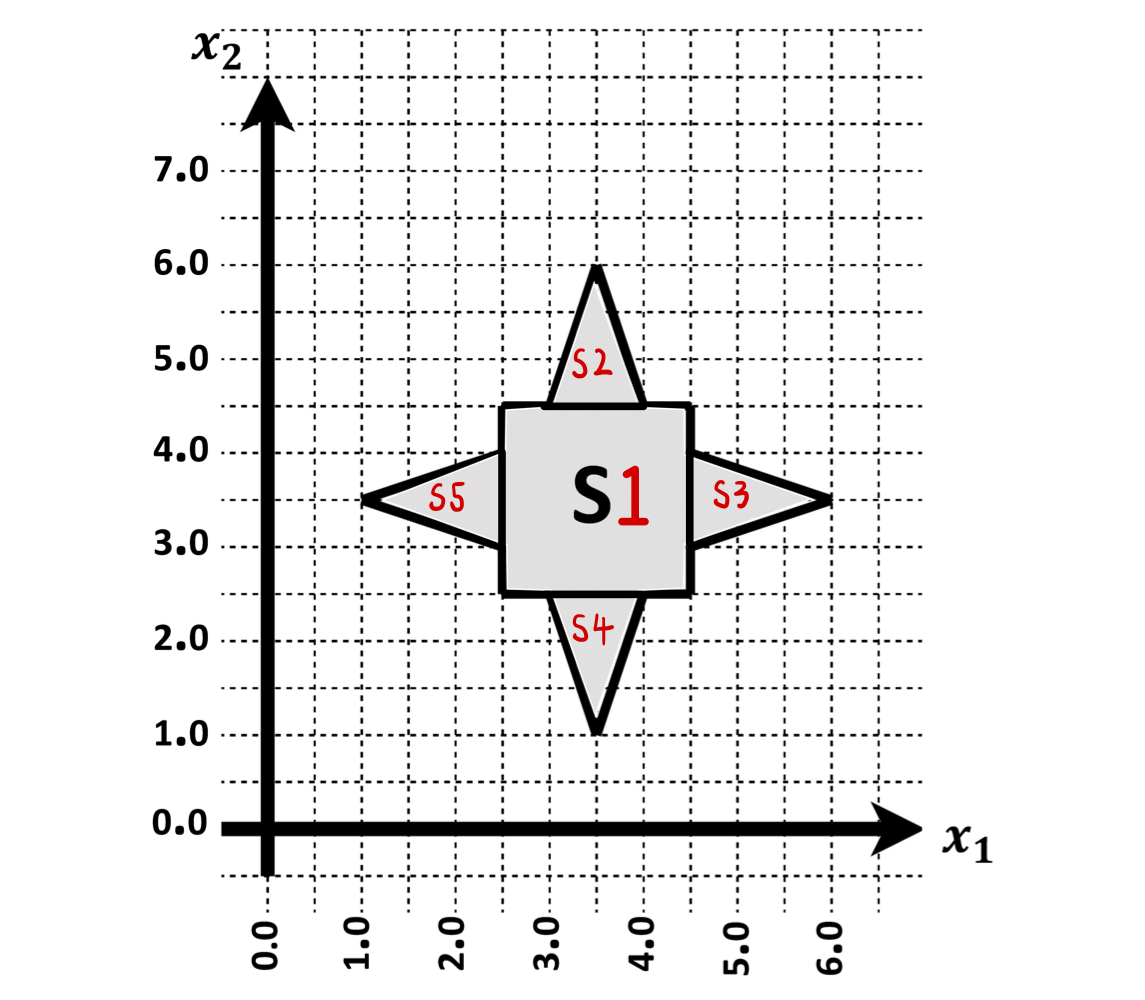
\includegraphics[width=8.5cm]{Prob7.2.png}
\caption{Figure 2}
\end{minipage}
\end{figure}

\item
It's obvious that Function F is meaningful only if it's region is convex. So to give this \textbf{ConvOpt} algorithm a qualified input, we need to divide the original region S into 5 small regions, which are all convex regions(as shown in figure2).


This way, we can use this \textbf{ConvOpt} algorithm to get 5 different results, which are respectively the minimum in their region. Then we choose the minimum among this 5 values, it is the minimum of whole region S.

\end{enumerate}
\end{document}
